\section{Import atomic structure protocol}
\label{app:importAtomicStructure}%a080
Protocol designed to import an atomic structure in \scipion from PDB database or from a file of computer's user.
   
 \begin{itemize}
  \item \scipion menu:\\
  \ttt{Protocols SPA -> Imports} (\ffigure{fig:app_protocol_atomicStructure_1} (A))\\
  
  \item Protocol form parameters (\ffigure{fig:app_protocol_atomicStructure_1} (B)):\\
  
  \begin{figure}[H]
    \centering 
    \captionsetup{width=.7\linewidth} 
    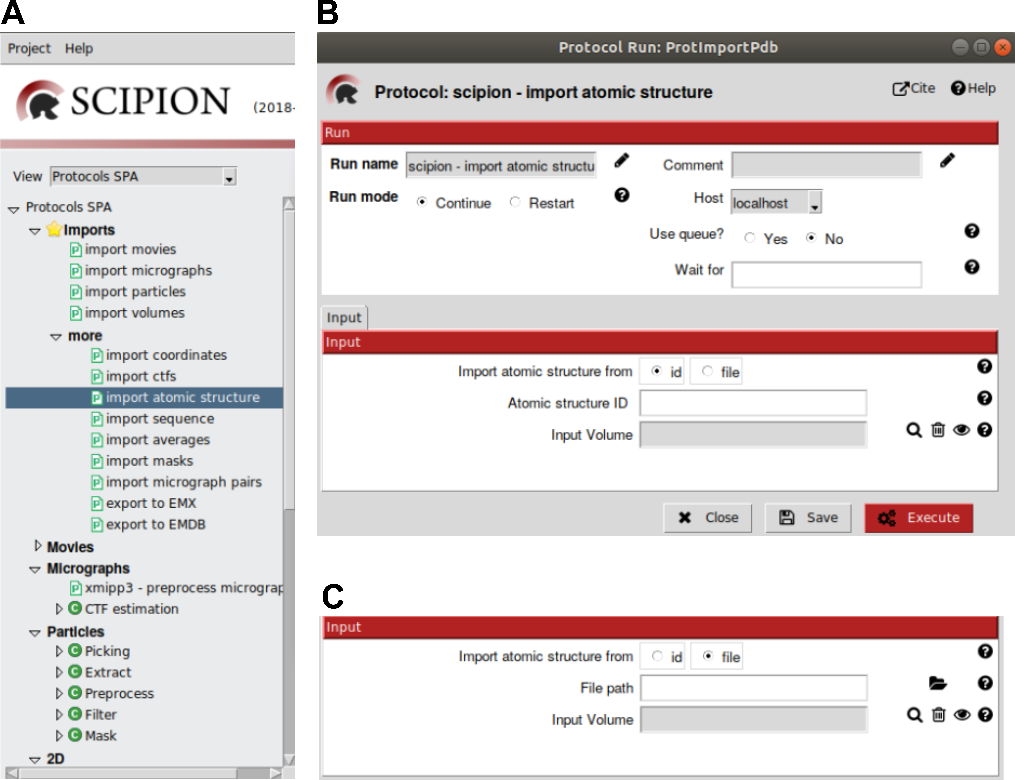
\includegraphics[width=0.90\textwidth]{Images_appendix/Fig110.pdf}
    \caption{Protocol \scommand{import atomic structure}. A: Protocol location in \scipion menu. B: Protocol form to import the atomic structure from PDB. C: Protocol form to import the atomic structure from a file.}
    \label{fig:app_protocol_atomicStructure_1}
   \end{figure}

  \begin{itemize}
   \item \ttt{Import atomic structure from}: Parameter to select the origin of the atomic structure that you want to import. Two options are indicated:\\
    \begin{itemize}
	 \item \ttt{id}: Select this option if you want to import the atomic structure from PDB database. Associated to this option is the next form parameter:\\
	  \begin{itemize}
	   \item \ttt{Atomic structure ID}: Box to write the accession ID of the desired PDB structure. Structure extension .cif/ .pdb. is not required.\\
	  \end{itemize}
	 \item \ttt{file}: Select this option if you want to import the atomic structure from a file. A new parameter appears associated to this option (\ffigure{fig:app_protocol_atomicStructure_1} (C)):\\
	  \begin{itemize}
	   \item \ttt{File path}: Box to be completed with the file path. The browser located at the right side of the parameter box helps to look for the file in the computer's user. \\
	  \end{itemize}
	\end{itemize}
   \item \ttt{Input Volume}: In case you want to associate a previously downloaded volume in \scipion to the atomic structure, you can select it here.\\
   \end{itemize}

  \item Protocol execution:\\
  
  Adding specific atomic structure label is recommended in \ttt{Run name} section, at the form top. To add the label, open the protocol form, press the pencil symbol at the right side of \ttt{Run name} box, complete the label in the new opened window, press OK, and finally close the protocol. This label will be shown in the output summary content (see below). If you want to run again this protocol, do not forget set to \ttt{Restart} the \ttt{Run mode}.\\
  Press the \ttt{Execute} red button at the form bottom.\\
  
  \item Visualization of protocol results:\\
  
  After executing the protocol, press \ttt{Analyze Results} and $Chimera$ graphics window will be opened by default (\ffigure{fig:app_protocol_volume_3}). 
  Atomic structures are referred to the origin of coordinates in \chimera. To show the relative position of the atomic structure, the three coordinate axes are represented; X axis (red), Y axis (yellow), and Z axis (blue). Coordinate axes and imported atomic structure are model numbers \ttt{\#0} and \ttt{\#1}, respectively, in $Chimera$ \ttt{Model Panel}. If a volume has been associated to the atomic structure, coordinate axes and imported atomic structure are model numbers \ttt{\#1} and \ttt{\#2}, respectively, in $Chimera$ \ttt{Model Panel}, whereas structure-associated volume has model number \ttt{\#0}. Volume coordinates and pixel size can be checked in $Chimera$ main menu \ttt{Tools -> Volume Data -> Volume Viewer -> Features -> Coordinates: Origin index/ Voxel size}. Take into account that coordinates appear in pixels while they have been introduced in \AA.\\
   
   \item Summary content:\\
    \begin{itemize}
     \item Protocol output (below \scipion framework):\\ \ttt{scipion - import structure -> ouputPdb}; \ttt{Pdbfile (pseudoatoms=True/ False, volume=True/ False)}.\\Pseudoatoms is set to \ttt{True} when the structure is made of pseudoatoms instead of atoms. Volume is set to \ttt{True} when an electron density map is associated to the atomic structure.\\
     \item \ttt{SUMMARY} box:\\Atomic structure imported from ID: \ttt{PDB accession ID}\\
    \end{itemize}

  \end{itemize}
